\documentclass[a4paper, 12pt]{article}

% --- 1. Page Layout & Typography ---
\usepackage[margin=1in]{geometry}
\usepackage{amsmath, amssymb}
\usepackage{parskip} % Adds space between paragraphs instead of indentation
\usepackage{times}   % Professional font (optional)

% --- 2. Header & Footer (Copyright Setup) ---
\usepackage{fancyhdr}
\pagestyle{fancy}
\fancyhf{} % Clear default header/footer

% Remove header line, keep footer line
\renewcommand{\headrulewidth}{0pt}
\renewcommand{\footrulewidth}{0.4pt}

% >>>> COPYRIGHT CONFIGURATION <<<<
\fancyfoot[L]{\footnotesize Copyright \copyright\ 2025 Your Name}
\fancyfoot[C]{\footnotesize \textit{Fundamental Theorem of Calculus}}
\fancyfoot[R]{\thepage}


% --- 3. TikZ Graphics Setup ---
\usepackage{tikz}
\usetikzlibrary{calc, decorations.pathreplacing, arrows.meta}


\title{\textbf{Calculus II: The Fundamental Theorem}}
\author{Your Name}
\date{\today}

\begin{document}
	
	\maketitle
	\thispagestyle{fancy} % Force copyright footer on the title page too
	
	\section{The Fundamental Theorem of Calculus (Part 2)}
	
	The second part of the theorem relates the definite integral of a derivative to the net change of the function:
	\[
	\int_a^b f'(x)\,dx = f(b) - f(a)
	\]
	
	\subsection*{Visual Proof}
	The visualization below demonstrates this relationship using the function $f(x) = \frac{1}{4}x^2 + 1$. 
	\begin{itemize}
		\item \textbf{Top Graph:} Shows the function $f(x)$. The tangent triangles illustrate the changing slope $f'(x)$. The brace shows the total vertical change.
		\item \textbf{Bottom Graph:} Shows the derivative $f'(x)$. The shaded area represents the accumulated sum of those slopes.
	\end{itemize}
	
	\vspace{1em}
	
	% --- BEGIN TIKZ FIGURE ---
	\begin{figure}[h!]
		\centering
		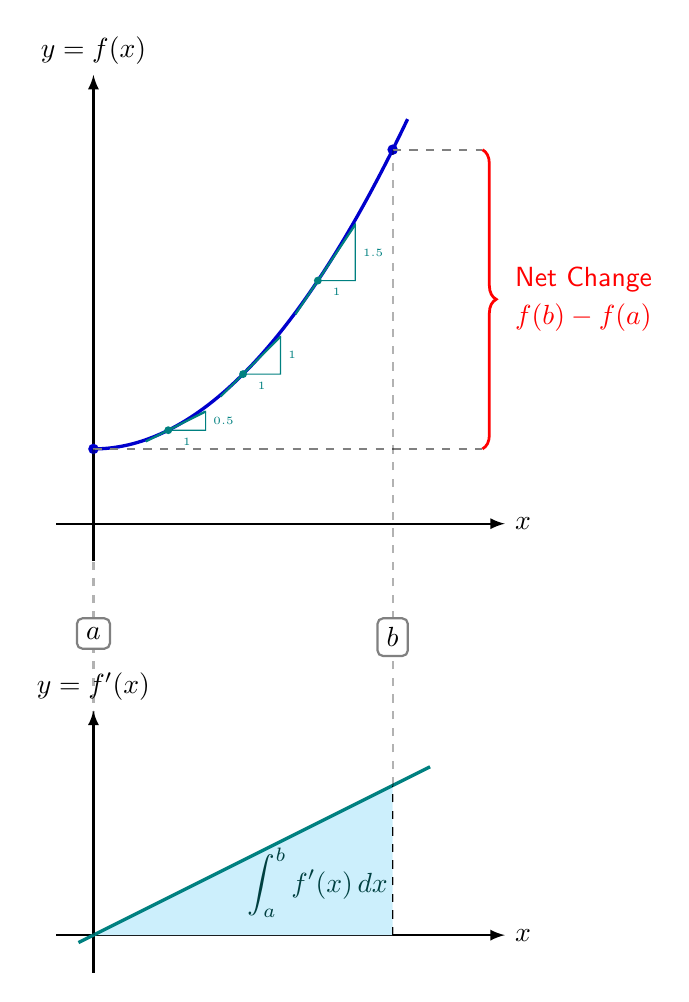
\begin{tikzpicture}[>=latex, font=\sffamily, thick, scale=0.95]
			
			% Constants
			\def\xa{0}
			\def\xb{4}
			\def\ysep{5.5} % Increased separation slightly for the document
			
			% Pre-calculations
			\pgfmathsetmacro{\ya}{0.25*\xa*\xa + 1}
			\pgfmathsetmacro{\yb}{0.25*\xb*\xb + 1}
			\pgfmathsetmacro{\yprimeb}{0.5*\xb}
			
			% === TOP GRAPH ===
			\begin{scope}[yshift=\ysep cm]
				\draw[->] (-0.5, 0) -- (5.5, 0) node[right] {$x$};
				\draw[->] (0, -0.5) -- (0, 6) node[above] {$y = f(x)$};
				\draw[blue!80!black, line width=1.2pt] plot[domain=0:4.2, samples=100] (\x, {0.25*\x*\x + 1});
				
				% Slope Triangles Loop
				\foreach \i in {1, 2, 3} {
					\pgfmathsetmacro{\ix}{\i}
					\pgfmathsetmacro{\iy}{0.25*\ix*\ix + 1}
					\pgfmathsetmacro{\slope}{0.5*\ix}
					\pgfmathsetmacro{\run}{0.5}
					\pgfmathsetmacro{\rise}{\slope*\run}
					
					\draw[teal, thin] 
					(\ix, \iy) -- (\ix + \run, \iy) node[midway, below, font=\tiny, scale=0.8] {1} 
					-- (\ix + \run, \iy + \rise) node[midway, right, font=\tiny, scale=0.8] {$\pgfmathprintnumber{\slope}$}
					-- cycle;
					\draw[teal, thick] (\ix, \iy) -- (\ix - 0.3, \iy - \slope*0.3);
					\draw[teal, thick] (\ix, \iy) -- (\ix + \run, \iy + \rise);
					\fill[teal] (\ix, \iy) circle (1.5pt);
				}
				
				\fill[blue!80!black] (\xa, \ya) circle (2pt);
				\fill[blue!80!black] (\xb, \yb) circle (2pt);
				\draw[dashed, gray] (\xa, \ya) -- (5.2, \ya);
				\draw[dashed, gray] (\xb, \yb) -- (5.2, \yb);
				\draw[decorate, decoration={brace, amplitude=5pt, mirror}, red, line width=1pt]
				(5.2, \ya) -- (5.2, \yb) node[midway, right=8pt, align=left] {Net Change\\[0.2em] $f(b) - f(a)$};
			\end{scope}
			
			% === BOTTOM GRAPH ===
			\begin{scope}
				\draw[->] (-0.5, 0) -- (5.5, 0) node[right] {$x$};
				\draw[->] (0, -0.5) -- (0, 3) node[above] {$y = f'(x)$};
				\fill[cyan!20] (\xa, 0) -- plot[domain=\xa:\xb] (\x, {0.5*\x}) -- (\xb, 0) -- cycle;
				\draw[teal, line width=1.2pt] (-0.2, -0.1) -- (4.5, 2.25);
				\node[teal!50!black] at (3, 0.7) {$\displaystyle \int_a^b f'(x)\,dx$};
				\draw[dashed, thin] (\xb, 0) -- (\xb, \yprimeb);
			\end{scope}
			
			% === CONNECTORS ===
			\draw[dashed, opacity=0.3] (\xa, 0) -- (\xa, \ya+\ysep);
			\draw[dashed, opacity=0.3] (\xb, 0) -- (\xb, \yb+\ysep);
			\node[below, draw=black!50, fill=white, rounded corners=2pt] at (\xa, 4.25) {$a$};
			\node[below, draw=black!50, fill=white, rounded corners=2pt] at (\xb, 4.25) {$b$};
			
		\end{tikzpicture}
		\caption{Geometric Interpretation of the Fundamental Theorem of Calculus.}
	\end{figure}
	% --- END TIKZ FIGURE ---
	
\end{document}